\section{Aufbau}
\label{sec:Aufbau}
In diesem Versuch wird ein Sagnac-Interferometer verwendet. Dieses ist in \autoref{fig:Sagnac}
schematisch dargestellt. 
\begin{figure}
    \centering
    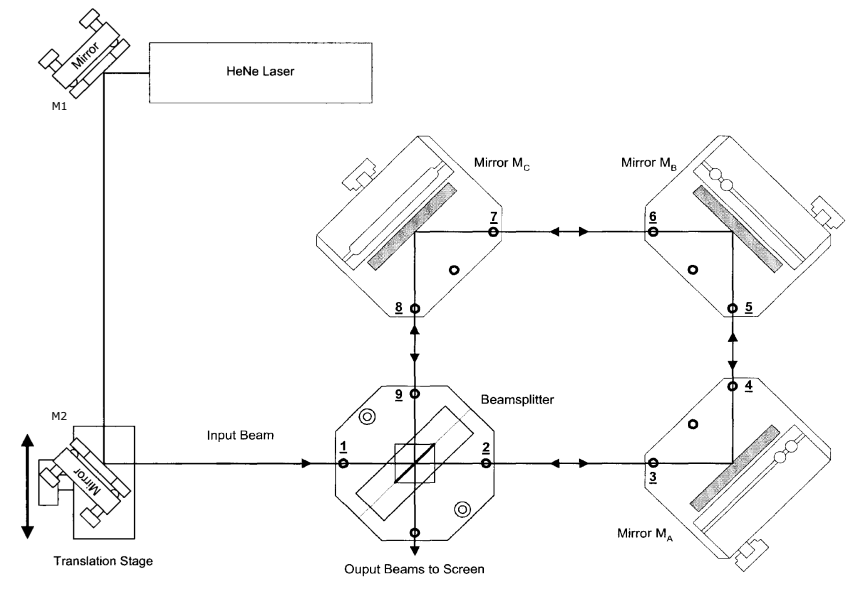
\includegraphics[width=0.8\textwidth]{Sagnac.png}
    \caption{Schematischer Aufbau eines Sagnac-Interferometers \cite{ap64}.}
    \label{fig:Sagnac}
\end{figure}
Das Interferometer besteht aus einem HeNe-Laser, der linear polarisiertes Licht der Wellenlänge $632.99\,\unit{\nano\meter}$
emittiert, und aus mehreren Spiegeln. Das Licht des Lasers ist in dessen Polarisation außerdem um 45° gegenüber der Vertikalen gekippt.
Die ersten beiden Spiegel M1 und M2 dienen dazu, den Laser in das Interferometer zu lenken. Die weiteren drei Spiegel $\symup{M_A}$, 
$\symup{M_B}$ und $\symup{M_C}$ sind Teil des Interferometers. Des Weiteren enthält es ein PBSC, der den Laserstrahl teilt.
Zur Justage liegen dem Versuch 2 Justageplatten sowie Metallplättchen bei. Außerdem stehen ein Schirm, ein 45°-Polarisationsfilter und ein um 45°-gedrehter
PBSC zur Verfügung. 
Für die Messung enthält der Versuch zwei verkippte dünne Glasplatten mit der Dicke $T=1\,\mathrm{mm}$, eine Gaszelle, Photodioden sowie
ein Oszilloskop.